\chapter{Einbinden von Grafiken, Sourcecode und Anforderungen}
\label{Kap3}

\section{Bilder}

Natürlich können auch Grafiken und Bilder eingebunden werden, siehe z.\,B. \autoref{Kap2:NasaRover}. Hierbei ist zu beachten, dass \LaTeX{} die Bilder automatisch positioniert, sie also nicht zwingend an der Stelle erscheinen, an der sie im Quelltext vorkommen (man spricht hier von \enquote{floats}). Das ist vollkommen in Ordnung und im Sinne einer ausgeglichenen Typografie auch sinnvoll.

\begin{figure}[ht]
  \centering
  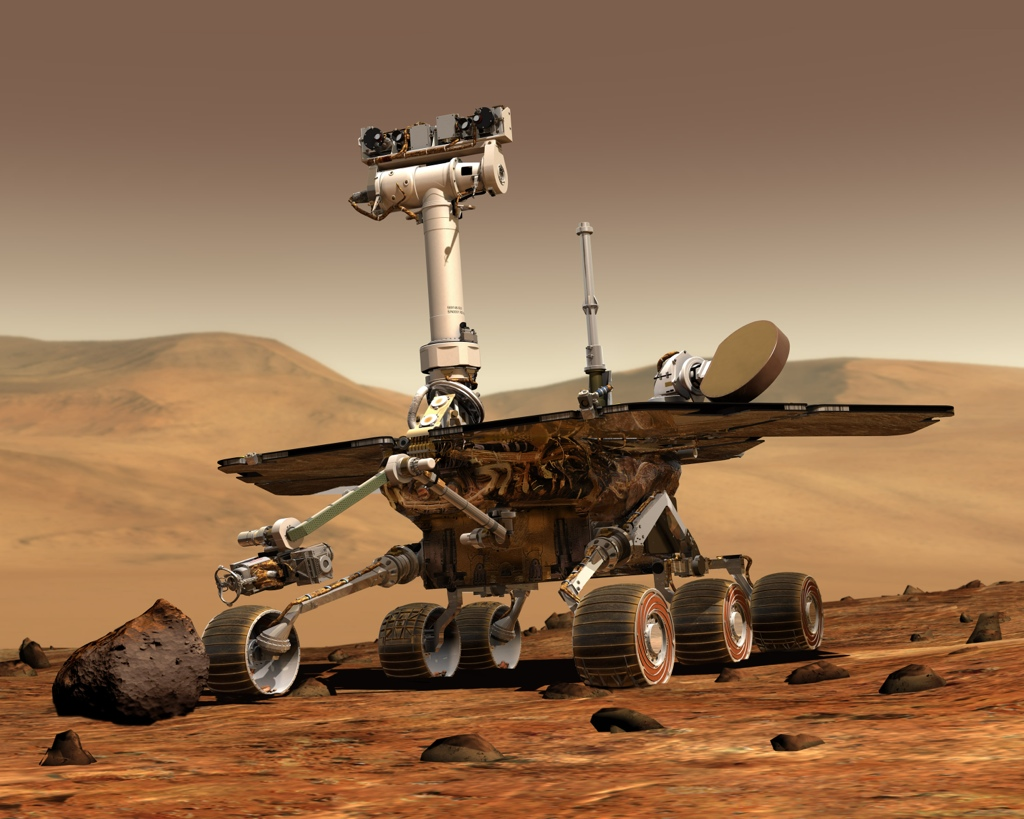
\includegraphics[width=6cm]{kapitel3/nasa_rover}
  \caption{Ein Nasa Rover}
  \label{Kap2:NasaRover}
\end{figure}

Man kann sich auch selbst ein Makro für das Einfügen von Bildern schreiben:

\bild{kapitel3/modell_point_to_point}{6cm}{Point to Point}

\begin{sidewaysfigure}
 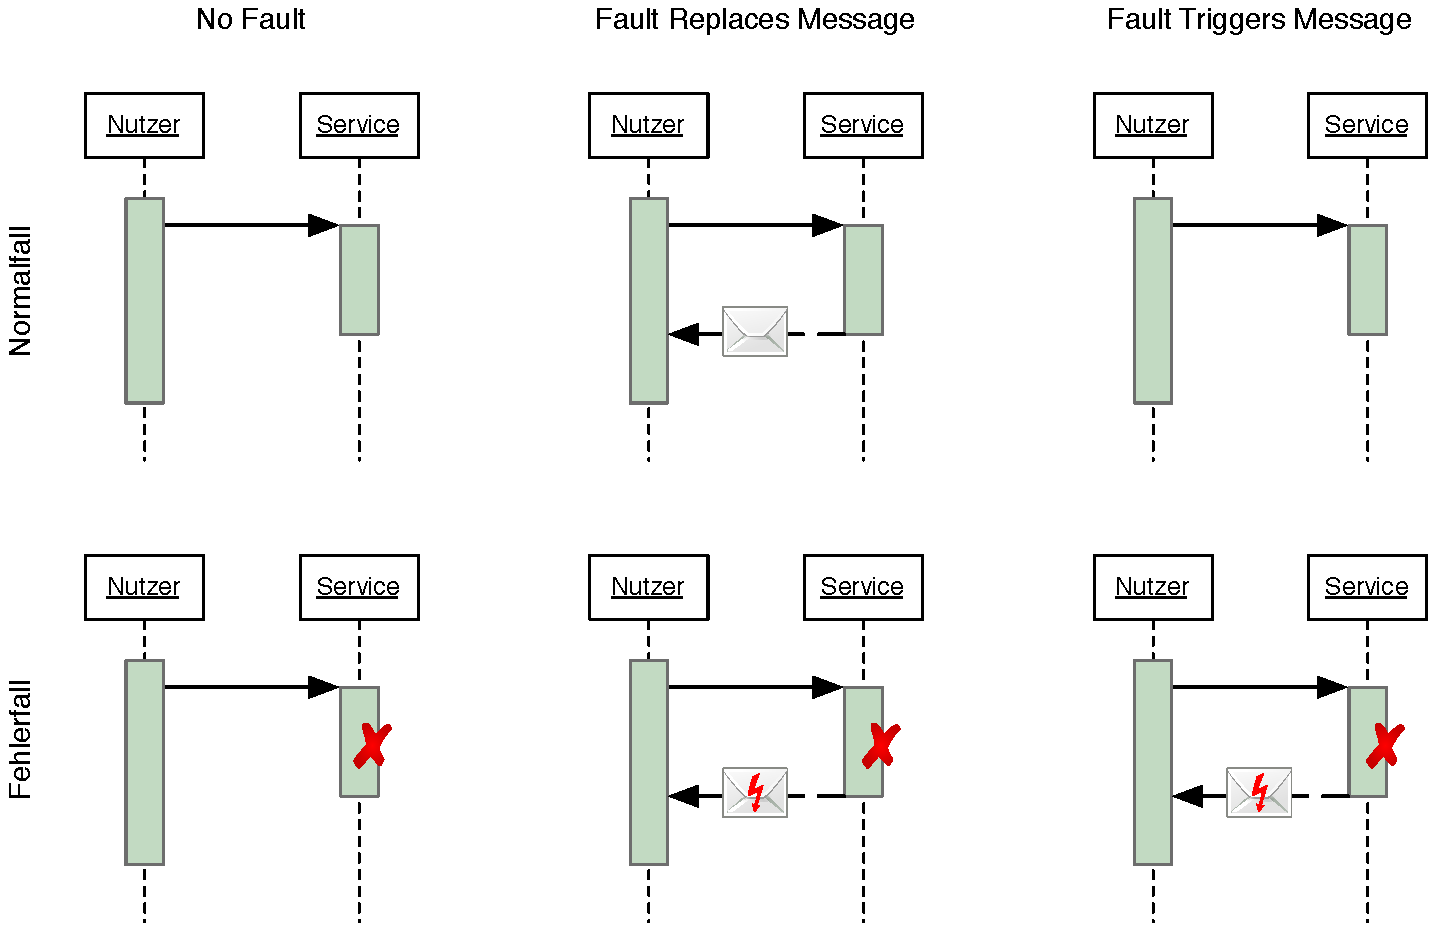
\includegraphics[width=22cm]{kapitel3/ws-wsdl20-fehler}
  \caption{Sehr große Grafiken kann man drehen, damit sie auf die Seite passen}
  \label{Kap2:wsdl-fehler}
\end{sidewaysfigure}

Möchte man verhindern, dass Bilder in ein anderes Kapitel rutschen, steht der Befehl \verb+\clearpage+ zur Verfügung, der \LaTeX{} zwingt, alle bis dahin definierten \textit{floats} (Bilder, Tabellen, Formeln etc.) auszugeben.

\clearpage % Alle Bilder, die bisher kamen ausgeben


\section{Formelsatz}

Eine Formel gefällig? Mitten im Text $a_2 = \sqrt{x^3}$ oder als eigener Absatz (siehe \autoref{Formel}):

\begin{equation}
\begin{bmatrix}
   1 &  4 &  2 \\
   4 &  0 & -3
\end{bmatrix}
        \cdot
\begin{bmatrix}
   1 &  1 &  0 \\
  -2 &  3 &  5 \\
   0 &  1 &  4
\end{bmatrix}
       {=}
\begin{bmatrix}
  -7 &  15 &  28 \\
   4 &   1 & -12
\end{bmatrix}
\label{Formel}
\end{equation}

Wenn Ihre Formel zu breit für eine Zeile wird, können Sie sie mithilfe der \texttt{split}-Umgebung und einem doppelten Backslash (\verb+\\+) umbrechen.

\begin{equation}
\label{eq:4}
\begin{split}
\mathbf{F}_{{eigen}}=\sqrt[3]{\coprod_{i=1}^{3} \lambda_{i}},
\frac{\lambda_{1}-\lambda_{3}}{\lambda_{1}},
\frac{\lambda_{2}-\lambda_{3}}{\lambda_{1}},
\frac{\lambda_{3}}{\lambda_{1}} \\-
\sum_{i=1}^{3} \lambda_{i} \log \left(\lambda_{i}\right),
\frac{\lambda_{1}-\lambda_{2}}{\lambda_{1}}
\end{split}
\end{equation}

Sie können Formelelemente auch am Gleichheitszeichen ausrichten, hierzu dient die \texttt{align}-Umgebung:

\begin{align}
2x - 5y &=  8 \\
3x + 92y &=  -12
\end{align}

Wollen Sie keine Nummerierung der Formeln, ergänzen Sie einfach einen \texttt{*} bei den Namen der Umgebungen, d.h. Sie verwenden \texttt{equation*} oder \texttt{align*}.

\begin{equation*}
\begin{bmatrix}
   1 &  4 &  2 \\
   4 &  0 & -3
\end{bmatrix}
        \cdot
\begin{bmatrix}
   1 &  1 &  0 \\
  -2 &  3 &  5 \\
   0 &  1 &  4
\end{bmatrix}
       {=}
\begin{bmatrix}
  -7 &  15 &  28 \\
   4 &   1 & -12
\end{bmatrix}
\end{equation*}


\section{Sourcecode}

Man kann mit Latex auch ganz toll Sourcecode in den Text aufnehmen.

\subsection{Aus einer Datei}

\lstinputlisting[firstline=2,                 % Erste anzuzeigende Zeile aus der Datei
                 language=Java,               % Programmmiersprache (für Highlighting)
                 caption={Crypter-Interface}, % Beschriftung
                 label=lst:CrypterInterface]  % Label (für Referenzen)
                 {\srcloc/Crypter.java}       % Pfad zur Datei, die angezeigt wird

Mit Zeilennummern

\lstinputlisting[numbers=left,                % Mit Zeilennummern auf der linken Seite
                 firstline=10,                % Erste anzuzeigende Zeile aus der Datei
                 lastline=15,                 % Letzte anzuzeigende Zeile aus der Datei
                 language=Java,               % Programmmiersprache (für Highlighting)
                 caption={Crypter},           % Beschriftung
                 label=lst:CrypterInterface2] % Label (für Referenzen)
                 {\srcloc/Crypter.java}       % Pfad zur Datei, die angezeigt wird


\subsection{Inline}

\begin{lstlisting}[language=Java,caption=Methode checkKey()]
    /**
     * Testet den Schlüssel auf Korrektheit: Er muss mindestens die Länge 1
     * haben und darf nur Zeichen von A-Z enthalten.
     *
     * @param key zu testender Schlüssel
     * @throws CrypterException wenn der Schlüssel nicht OK ist.
     */
    protected void checkKey(Key key) throws CrypterException {

        // Passt die Länge?
        if (key.getKey().length == 0) {
            throw new CrypterException("Der Schlüssel muss mindestens " +
                    "ein Zeichen lang sein");
        }

        checkCharacters(key.getKey(), ALPHABET);
    }
\end{lstlisting}


\section{Anforderungen}

Anforderungen im Format des Volere"=Templates (Snowcards) \autocite{Volere} können per Makro eingefügt werden. Das Label wird automatisch mit der Nummer erstellt, d.\,h. Sie können auf die Tabelle mit dieser referenzieren (siehe \autoref{F52}).

\snowcard % Snowcard einbinden (Anpassungen in titelblatt.tex)
   {F52} % Nummer des Requirements
   {F} % Art
   {Hoch} % Priorität
   {User Authentifizierung} % Titel
   {Interview mit Abteilungsleiter} % Herkunft (Optional)
   {F12} % Konflikte (Optional)
   {Der Benutzer ist in der Lage sich über seinen
    Benutzernamen und sein Passwort am System anzumelden} % Beschreibung
   {Ein Benutzer kann sich mit seinem firmenweiten Benutzernamen und
   Passwort über die Anmeldemaske anmelden und hat Zugriff auf die
   Funktionen des Systems} % Fit-Kriterium (Optional)
   {Benutzerhandbuch des Altsystems} % Material (Optional)

Ebenso können Sie nicht"=funktionale Anforderungen mit Hilfe von Quality Attribute Scenarios (vgl. \autoref{NF11}) darstellen. Zu Details siehe \autocite{Barbacci2003}.

\qas % Quality-Attribute Scenario einbinden (Anpassungen in titelblatt.tex)
   {NF11} % Nummer des Requirements
   {Hoch} % Priotität
   {Performance des Jahresabschlusses} % Titel
   {Endbenutzer} % Quelle
   {Startet einen Jahresabschluss} % Stimulus
   {Buchhaltungssystem} % Artefakt
   {Das System befindet sich im normalen Betriebszustand} % Umgebung
   {Jahresabschluss ist durchgeführt und kann als PDF abgerufen werden} % Antwort
   {10 Minuten} % Antwort-Maß

Die Abgrenzung von funktionalen und nicht-funktionalen Anforderungen ist nicht immer einfach und bereitet manchen Studierenden Probleme. Als Hilfestellung kann die von der ISO25010 \autocite{ISO25010} zur Verfügung gestellte Liste dienen, siehe \autoref{kapitel3/iso25010}.

\bild{kapitel3/iso25010}{14cm}{Qualitätsmodell für Software-Produkte nach ISO25010}

\citeauthor{Bass2003} listen in \autocite{Bass2003} eine ähnliche Liste von Kategorien für nicht-funktionalen Anforderungen auf, die ebenfalls als Richtschnur dienen kann. Diese sind:

\begin{itemize}
  \item \textit{Verfügbarkeit} \textit{(availability)} -- umfasst Zuverlässigkeit (reliability), Robustheit (robustness), Fehlertoleranz (fault tolerance) und Skalierbarkeit (scalability)
  \item \textit{Anpassbarkeit} \textit{(modifiability)}, umfasst Wartbarkeit (maintainability), Verständlichkeit (understandability) und Portabilität (portability).
  \item \textit{Performanz} \textit{(performance)}
  \item \textit{Sicherheit} \textit{(security)}
  \item \textit{Testbarkeit} \textit{(testability)}
  \item \textit{Bedienbarkeit} \textit{(usability)}
\end{itemize}
